\documentclass[fleqn, a4paper, 12pt]{article}
\usepackage{amsmath, amssymb, amsthm}
\usepackage{gensymb}
\usepackage{commath}
\usepackage{xcolor}
\usepackage{cancel}
\usepackage{siunitx}
\usepackage{tikz, pgfplots}
	\usetikzlibrary{calc, hobby, patterns, intersections}
\usepackage{graphicx}
\usepackage{hyperref}
\usepackage{datetime}
\usepackage{ulem}
\usepackage{xfrac}
\usepackage{asymptote}
\usepackage{enumerate}
\setcounter{secnumdepth}{4}
\newcommand\numberthis{\addtocounter{equation}{1}\tag{\theequation}}

\newcommand{\AxisRotator}[1][rotate=0]{%
	\tikz [x=0.25cm,y=0.60cm,line width=.2ex,-stealth,#1] \draw (0,0) arc (-150:150:1 and 1);%
}

\theoremstyle{definition}
\newtheorem{example}{Example}
\newtheorem{definition}{Definition}

\theoremstyle{theorem}
\newtheorem{theorem}{Theorem}

\newenvironment{solution}
{\begin{proof}[Solution]\let\qed\relax}
	{\end{proof}}

\newcommand{\curl}{\mathrm{curl\,}}

%\renewcommand{\int_{min}^{max}}{\int\displaylimits_{min}^{max}}

%opening
\title{Lecture 19}
\author{Aakash Jog}
\date{\formatdate{1}{1}{2015}}

\begin{document}

\maketitle
%\setlength{\mathindent}{0pt}

\tableofcontents

\newpage
\section{Rigid Body Mechanics}

\begin{example}
	A string is wound around a pulley of mass $m_1$ and radius $R_1$, which is fixed at its centre. The other end of the string is wound onto another pulley of mass $m_2$ and radius $R_2$. The string unwinds and the second pulley moves vertically downwards. Find the acceleration of the second pulley.\\
	\begin{tikzpicture}
		\def\1R{3};
		\def\2R{2};
		\def\l{5};
		\def\angle{30};
		
		\coordinate(pulley 1 centre) at (0,0);
		\coordinate(pulley 1 right) at ($ (pulley 1 centre) + (0:\1R) $);
		
		\coordinate(pulley 2 left) at ($ (pulley 1 right) + (-90:\l) $);
		\coordinate(pulley 2 centre) at ($ (pulley 2 left) + (0:\2R) $);
		
		\draw (pulley 1 centre) circle [radius = \1R];
		\draw [dashed] (pulley 1 centre) -- ++(\angle:\1R) node [midway, fill = white] {$R_1$};
		
		\draw (pulley 2 centre) circle [radius = \2R];
		\draw [dashed] (pulley 2 centre) -- ++(\angle:\2R) node [midway, fill = white] {$R_2$};
		
		\draw (pulley 1 right) -- (pulley 2 left);
	\end{tikzpicture}
\end{example}

\begin{solution}
	For $m_1$, about its centre,
	\begin{align*}
		T R_1 &= I_{O,1} \alpha_1\\
		&= \dfrac{1}{2} m_2 {R_1}^2 \alpha_1\\
		\therefore T &= \dfrac{1}{2} m_1 R_1 \alpha_1
	\end{align*}
	For $m_1$,
	\begin{align*}
		m_2 g - T &= m_2 a_2
	\end{align*}
	For $m_2$, about its centre,
	\begin{align*}
		T R_2 &= \dfrac{1}{2} m_2 {R_2}^2 \alpha_2\\
		\therefore T &= \dfrac{1}{2} m_2 R_2 \alpha_2
	\end{align*}
	As the second pulley goes down vertically, the string is being unwound from both pulleys. Therefore,
	\begin{align*}
		a_2 &= \alpha_1 R_1 + \alpha_2 R_2
	\end{align*}
\end{solution}

\subsection{Gyroscope}
A disk is attached to rods as shown, and is rotating about itself with $\omega$.
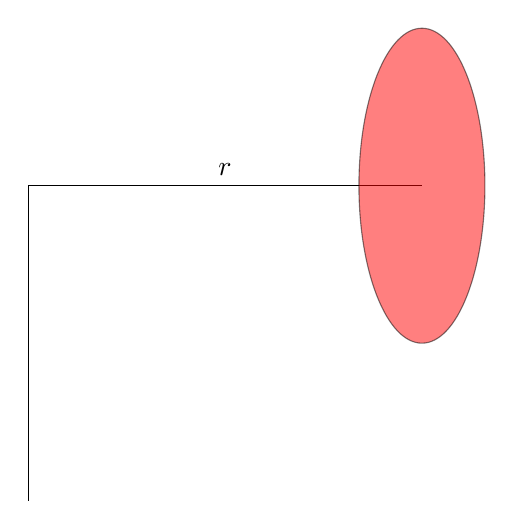
\begin{tikzpicture}
	\def\y{4};
	\def\x{5};
	\def\R{2};

	\draw (0,0) -- (0,\y);
	\draw (0,\y) -- (\x,\y) node [midway, above] {$r$};
	
	\filldraw [fill = red, opacity = 0.5] (\x,\y) circle [x radius = 0.4*\R, y radius = \R];
\end{tikzpicture}\\
The torque is directed $\otimes$.\\
Seen from the top,\\
\begin{tikzpicture}
	\def\r{4};
	\def\R{1};
	\def\angle{30};
	\def\F{1};
	
	\draw (0,0) -- (\angle:\r) node [midway, above] {$r$};
	\draw [ultra thick, red] (\angle:\r) -- ++({90 + \angle}:\R);
	\draw [ultra thick, red] (\angle:\r) -- ++({-90 + \angle}:\R);
	
	\draw [-stealth] (0,0) -- ++({90 + \angle}:\F) node [above] {$\tau$};
	\draw [-stealth] (\angle:\r) -- ++(\angle:\F) node [above] {$L$};
\end{tikzpicture}\\
\begin{align*}
	\overrightarrow{\tau} &= \tau \hat{\theta}
\end{align*}
with respect to the joint,
\begin{align*}
	\overrightarrow{L} &= \dfrac{1}{2} m R^2 \omega \hat{r}\\
	\therefore \dod{\overrightarrow{L}}{t} &= \dfrac{1}{2} m R^2 \omega \cdot \dod{\hat{r}}{t}\\
	\therefore \tau &= \dfrac{1}{2} m R^2 \omega \dot{\theta}\\
	\therefore m g r &= \dfrac{1}{2} m R^2 \omega \dot{\theta}
\end{align*}
Therefore,
\begin{align*}
	\dot{\theta} &= \dfrac{2 g r}{R^2 \omega}
\end{align*}

\begin{example}
	A disk of mass $m$ and radius $R$ is fixed on a rod and is kept on two stands fixed on another disk which is rotating with $\Omega$. Find the normal forces that the stands are exerting on the rod.\\
	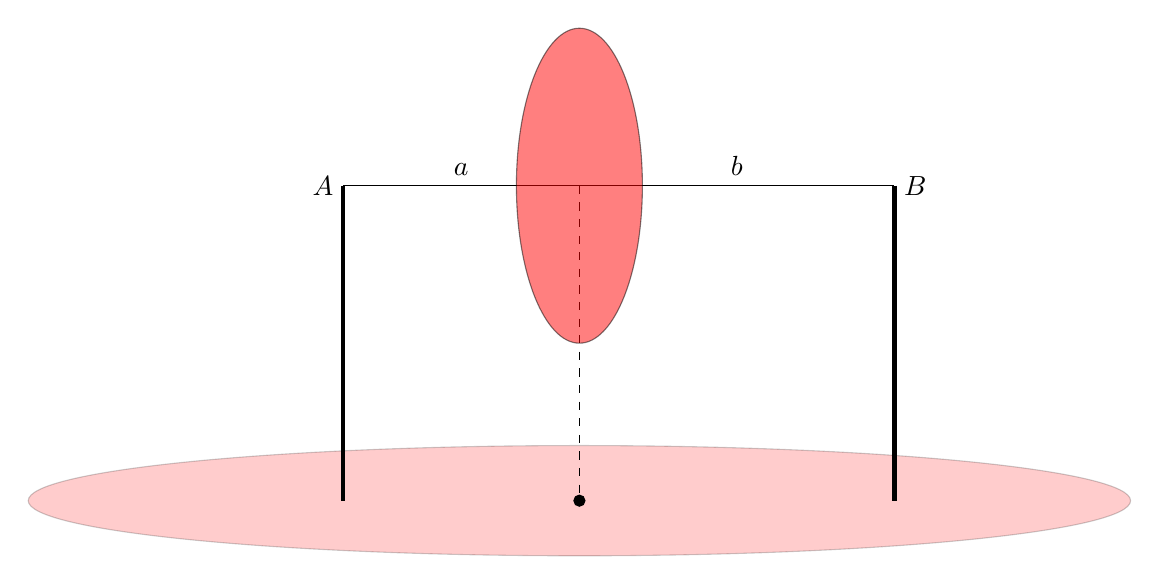
\begin{tikzpicture}
		\def\z{4};
		\def\a{3};
		\def\b{4};
		\def\R{2};
		
		\coordinate (disk centre) at (0,\z);
		\coordinate (A) at (-\a,\z);
		\coordinate (B) at (\b,\z);

		\filldraw [fill = red, opacity = 0.2] (0,0) circle [x radius = {\a + \b}, y radius = {0.1*(\a + \b)}];
		
		\filldraw (0,0) circle [radius = 2pt];
		
		\draw [ultra thick] (A) -- ++(-90:\z);
		\draw [ultra thick] (B) -- ++(-90:\z);
		
		\node at (A) [left] {$A$};
		\node at (B) [right] {$B$};
		
		\draw (disk centre) -- (A) node [midway, above] {$a$};
		\draw (disk centre) -- (B) node [midway, above] {$b$};
		
		\draw [dashed] (disk centre) -- (0,0);
		
		\filldraw [fill = red, opacity = 0.5] (0,\z) circle [x radius = 0.4*\R, y radius = \R];
	\end{tikzpicture}\\
	\begin{tikzpicture}
		
	\end{tikzpicture}
\end{example}

\begin{solution}
	As viewed from the top,\\
	\begin{tikzpicture}
		\def\angle{30};
		\def\a{4};
		\def\b{4};
		\def\F{3};
		
		\draw [-stealth, red] (0,0) -- (\angle:1) node [above] {$\hat{r}$};
		
		\draw [-stealth, red] (0,0) -- ({90 + \angle}:1) node [above right] {$\hat{\theta}$};
		
		\draw [dashed] (0,0) -- (\angle:\b) node [above right] {$N_B$};
			\node at (\angle:\b) {$\odot$};
		
		\draw [dashed] (0,0) -- ({180 + \angle}:\a) node [above left] {$N_A$};
			\node at ({180 + \angle}:\a) {$\odot$};
		
		\draw [-stealth] (0,0) -- (\angle:\F) node [above] {$L$};
		\draw [-stealth] (0,0) -- ({90 + \angle}:\F) node [above] {$\tau_A$};
		\draw [-stealth] (0,0) -- ({-90 + \angle}:\F) node [below] {$\tau_B$};
	\end{tikzpicture}\\
	About the point $O$,
	\begin{align*}
		\overrightarrow{L} &= \dfrac{1}{4} m R^2 \Omega \hat{z} + \dfrac{1}{2} m R^2 \omega \hat{r}\\
		\therefore \overrightarrow{\tau} &= \dod{\overrightarrow{L}}{t}\\
		&= \dod{}{t} \left( \dfrac{1}{4} m R^2 \Omega \hat{z} + \dfrac{1}{2} m R^2 \omega \hat{r} \right)\\
		&= \dod{}{t} \left( \dfrac{1}{2} m R^2 \omega \hat{r} \right)
	\end{align*}
	The net torque about point $O$ is only due to the normal forces.\\
	Therefore, the net torque is in the $\hat{\theta}$ direction. Hence, it cannot change the magnitude of $\omega$, but only the direction.\\
	Therefore,
	\begin{align*}
		\overrightarrow{\tau} &= \dod{}{t} \left( \dfrac{1}{4} m R^2 \Omega \hat{z} + \dfrac{1}{2} m R^2 \omega \hat{r} \right)\\
		&= \dfrac{1}{2} m R^2 \omega \dod{\hat{r}}{t}\\
		&= \dfrac{1}{2} m R^2 \omega \dot{\theta} \hat{\theta}\\
		&= \dfrac{1}{2} m R^2 \omega \Omega \hat{\theta}\\
		\therefore a N_A \hat{\theta} + b N_b (-\hat{\theta}) &= \dfrac{1}{2} m R^2 \omega \Omega \hat{\theta}
	\end{align*}
	Therefore,
	\begin{align*}
		a N_A - b N_B &= \dfrac{1}{2} m R^2 \omega \Omega
	\end{align*}
	Also,
	\begin{align*}
		N_A + N_B &= m g
	\end{align*}
\end{solution}

\section{Second Order Linear Differential Equations with Constant Coefficients}

\subsection{Homogeneous Differential Equations}

\begin{align*}
	a y'' + b y' + c &= 0\\
	\intertext{Let $y = e^{\lambda x}$}
	\therefore a \lambda^2 + b \lambda + c &= 0\\
	\therefore \lambda &= \dfrac{-b \pm \sqrt{b^2 - 4 a c}}{2 a}
\end{align*}
If $\Delta > 0$,
\begin{align*}
	y &= A e^{\lambda_1 x} + B e^{\lambda_2 x}
\end{align*}
is the general solution to the differential equation.\\
If $\Delta < 0$,
\begin{align*}
	y &= e^{\alpha x} \left( C \cos (\beta x) + D \sin (\beta x) \right)
\end{align*}
is the general solution to the differential equation.\\
If $\Delta = 0$,
\begin{align*}
	y &= A e^{\lambda x} + B x e^{\lambda  x}
\end{align*}
is the general solution to the differential equation.

\section{Simple Harmonic Oscillator}

A mass $m$ is attached to a spring of coefficient $k$, which is at its natural length. The spring is stretched by $x$ and released.
\begin{align*}
	x(t = 0) &= A\\
	\dot{x}(t = 0) &= 0
\end{align*}
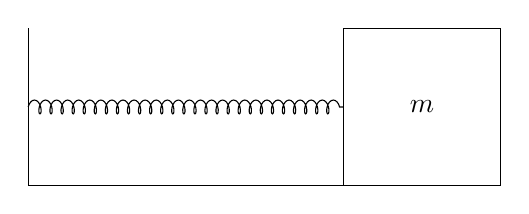
\begin{tikzpicture}
	\def\l{4};
	\def\x{1};
	\def\segmentlength{4};
		
	\draw (0,2) -- (0,0) -- (\l,0);
		
	\draw [decorate, decoration = {coil, segment length = \segmentlength}](0,1) -- (\l,1);
	
	\draw (\l,2) rectangle  node {$m$} ({\l + 2}, 0);
\end{tikzpicture}\\
\vspace{1in}\\
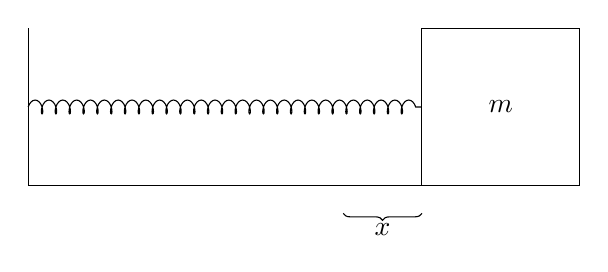
\begin{tikzpicture}
	\def\l{4};
	\def\x{1};
	\def\segmentlength{4};
	
	\draw (0,2) -- (0,0) -- ({\l + \x},0);
	
	\draw [decorate, decoration = {coil, segment length = {(\l + \x)/(\l)*\segmentlength}}](0,1) -- ({\l + \x},1);
	
	\draw ({\l + \x},2) rectangle  node {$m$} ({\l + \x + 2}, 0);
	
	\draw [decorate, decoration = {mirror, brace}, yshift = -10] (\l,0) -- ({\l + \x},0) node [midway, below] {$x$};
\end{tikzpicture}\\
\begin{align*}
	m \ddot{x} &= - k x\\
	\therefore \ddot{x} + \dfrac{k}{m} x &= 0
\end{align*}
Therefore, the characteristic equation is
\begin{align*}
	\lambda^2 + \dfrac{k}{m} &= 0\\
	\therefore \lambda &= \pm i \sqrt{\dfrac{k}{m}}
\end{align*}
Therefore,
\begin{align*}
	x &= C \cos \left( \sqrt{\dfrac{k}{m}} t \right) + D \sin \left( \sqrt{\dfrac{k}{m}} t \right)\\
	\therefore \dot{x} &= \sqrt{\dfrac{k}{m}} \left( - C \sin \left( \sqrt{\dfrac{k}{m}} t \right) + D \cos \left( \sqrt{\dfrac{k}{m}} t \right)\right)
\end{align*}
Solving with initial conditions,
\begin{align*}
	x &= A \cos \left( \sqrt{\dfrac{k}{m}} t \right)\\
	\dot{x} &= -A \sqrt{\dfrac{k}{m}} \sin \left( \sqrt{\dfrac{k}{m}} t \right)
\end{align*}
Alternatively, as the mechanical energy is constant throughout,
\begin{align*}
	E &= \dfrac{1}{2} m (\dot{x})^2 + \dfrac{1}{2} k x^2\\
	\therefore \dot{E} &= 0\\
	\therefore 0 &= \dfrac{1}{2} m (2 \dot{x}) \ddot{x}+ \dfrac{1}{2} k (2x) \dot{x}\\
	\therefore 0 &= \dot{x} \left( m \ddot{x} + k x \right)\\
	\therefore \ddot{x} + \dfrac{k}{m} x &= 0
\end{align*}

\begin{definition}[Angular frequency]
	The angular frequency is defined as
	\begin{align*}
		\omega_0 &= \sqrt{\dfrac{k}{m}}
	\end{align*}
\end{definition}

\end{document}